\chapter{Introduction, Spark and MapReduce} 
\section{MapReduce: Early Distributed Computing Programming Model} 
In general, MapReduce is a style of programming designed for 
    \begin{itemize}
        \item Easy parallel programming 
        \item Invisible management of hardware and software failures
        \item Easy management of very-large-scale data
    \end{itemize}
Some common implementations of MapReduce includes Hadoop, Spark, Flink, and the original Google implementation "MapReduce". 

\subsection{Component of MapReduce} 
The MapReduce framework has the following steps (note that user only needs to write map function and reduce function)
    \begin{enumerate}
        \item Map: Apply a user-written Map function to each input element. 
            \begin{itemize}
                \item Mapper applies the Map function to a single element
                \item Many mappes grouped in a Map task (the unit of parallelism)
                \item The output of the Map function is a set of 0, 1, or more key-valued pairs
                \item The keys do not have to be unique. A Map task can produce several key-value pairs with the same key even from the same element. 
            \end{itemize}
        \item Group by Key: Sort and shuffle 
            \begin{itemize}
                \item System sorts all the key-value pairs by key, and output key - (list of values) pairs
            \end{itemize}
        \item Reduce : User-written Reduce function is applied to each key - (list of values). The output is another sequence of zero or more key-value pairs. 
    \end{enumerate}
The MapReduce environment will automatically takes care of 
    \begin{itemize}
        \item Partitioning the input data
        \item Scheduling the program's execution across a set of machines
        \item Performing the group by key step 
        \item Handling machine failures
        \item Managing required inter-machine communication
    \end{itemize}

\paragraph{Quick Example: Word Count}\mbox{}\\
Task: We have a huge text document, and we need to count the number of times each distinct word appears in the file. The map function reads the input and produces a set of key-value pairs where the key is a word, and the value is 1. The reduce function is the sum function. (Note that because the Reduce function is associative and communicative, we can push some of the reducers work, addition, to the Map task. So the key is a word, but the value from Map function could be more than 1). 



\subsection{MapReduce and Machine Failures} 
If map worker failure: 
    \begin{itemize}
        \item Map tasks completed or in-progress at worker are reset to idle and rescheduled 
        \item Reduce workers are notified when map task is rescheduled on another worker
    \end{itemize}
If reduce worker failure: 
    \begin{itemize}
        \item Only in-progress tasks are reset to idle and the reduce task is restarted. 
    \end{itemize}



\subsection{Algorithms Using MapReduce} 
\subsubsection{Matrix-Vector Multiplication} 
Setup: \\
A $n \times n$ matrix $M$ and a vector $v$ of length $n$. We want to calculate $x = Mv$ where $x_i = \sum_{j=1}^n m_{ij}v_j$. We assuming that $m_{ij}$ and $v_j$ are discoverable by their coordinate $i,j$.We also assume $v$ can be read into memory in its entirety. \\

Map: \\
For each matrix element $m_{ij}$, it produces the key-value pair $(i. m_{ij}v_j)$. \\

Reduce: \\
The Reduce function simply sums all the values with a given key $i$. 

\subsubsection{Matrix-Vector Multiplication with large vector} 
Setup: \\
If $v$ is too large to fit into the memory, we slice $M$ vertically and $v$ horizontally in the same fashion. We can then divide $M$ and $v$ into different files where each files contains a set of stripes. See example in figure \ref{fig:mat_vec_div}. We can then proceed normally with Map and Reduce. 

\begin{figure}[h]
    \centering
    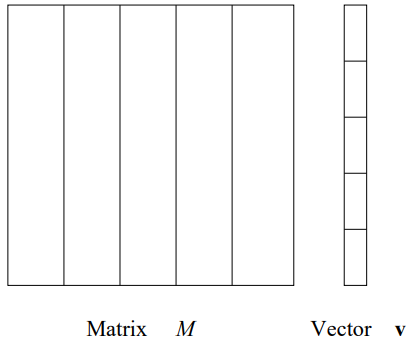
\includegraphics[width=4cm, height = 3cm]{figs/001_mat_vec_div.PNG}
    \caption{Division of a matrix and vector into five stripes}
    \label{fig:mat_vec_div}
\end{figure}

\subsubsection{Relational-Algebra Operations: Selection}
Task: Apply a condition $C$ to each tuple in the relation(a table) and produce as output only those tuples that satisfy $C$. Result is labeled as $\sigma_C(R)$. \\

Map: For each tuple $t$ in $R$, test if it satisfies $C$. If so, produce the key value pair $(t, t)$, otherwise produce nothing. \\

Reduce: Identity function. 

\subsubsection{Relational-Algebra Operations: Projection} 
Task: For some subset $S$ of the attributes of the relation, produce from each tuple only the components for the attributes in $S$. Result is labeled as $\pi_S(R)$.\\

Map: For each tuple $t$ in $R$, construct a tuple $t'$ by eliminating from $t$ those components whose attributes are not in $S$. Output key-value pair $(t', t')$\\

Reduce: Identity function. 

\subsubsection{Relational-Algebra Operations: Union}
Map: Turn each input tuple $t$ into key-value pair $(t,t)$ regardless which relation it comes from. \\

Reduce: Produce $(t, t)$ regardless the input value is $(t, [t])$ or $(t, [t, t])$. 

\subsubsection{Relational-Algebra Operations: Intersection} 
Map: Turn each input tuple $t$ into key-value pair $(t,t)$ regardless which relation it comes from. \\

Reduce: Produce $(t, t)$ only if the input value is $(t, [t, t])$. 

\subsubsection{Relational-Algebra Operation: Difference} 
Task: $R - S$. \\

Map: Produce key-value pair $(t, X)$ where $X$ can be either $R$ or $S$ based on where the input tuple is. \\

Reduce: Produce $(t, t)$ only if the input value $(t, [R])$. e.g.: $(t, [R,S])$ means that the tuple exists in both relation. 

\subsubsection{Relational-Algebra Operation: Natural Join} 
Task: Inner join $R(A,B)$ with $S(B,C)$ on shared attributes $B$. \\

Map: For each tuple $(a,b)$ of $S$, produce the key-value pair $(b, (R,a)$. Produce $(b, (S,c)$ for tuple in $S$. \\

Reduce: Input is $(b, (R,a), (S,c), (R,a'), (S,c'),...$. Output: pairwise across $R$ and $S$, and add $b$. So $(x, (b,a,c), (b,a',c),...)$. Here key is $x$ because it doesn't matter. 

\subsubsection{Relational-Algebra Operation: Grouping and Aggregation} 
Task: Group by attribute $A$, aggregating over attribute $B$ and left over attribute $C$. \\

Map: For each tuple $(a,b,c)$, produce key-value pair $(a,b)$. \\

Reduce: The aggregation function. 

\subsubsection{Matrix Multiplication - Two Step} 
Task: calculate $P = MN$ where $p_{ik}=\sum_j m_{ij}n_{jk}$. We can think of $MN$ as a natural join followed by grouping and aggregation. The natural join is $M(I, J, V)$ with $N(J,K,W)$. This will gives us tuples $(i, j, k, v \times w)$. Subsequently we can group by $I, K$ and aggregate over $J$. 

\subsubsection{Matrix Multiplication - One Step} 

Map: For each element $m_{ij}$ of $M$, produce all the key-value pairs $((i,k), (M,i,m_{ij}))$ for $k=1,2,...$ up to number of columns of $N$. For each element $n_{jk}$ of $N$, produce all the key-value pairs $((i,k),(N,j,n_{jk}))$ for $i=1,...$ up to the number of rows of $M$. \\

Reduce: Each key $(i,k)$ will have an associated list with all the values $(M,j,m_{ij})$ and $(N,j, n_{jk})$ for all possible values of $j$. The Reduce function connects two values on the list with the same $j$, and multiply $m_{ij}$ with $n_{jk}$ followed by summing at the key $(i,k)$ level. 
 
 
\section{Spark: Extends MapReduce} 

\subsection{Data-Flow Systems} 
MapReduce uses two ranks of tasks (Map, Reduce), and the data flows from the first rank to the second. Data-Flow Systems generalize this process by 1) Allowing any number of tasks / ranks, and 2) Allow functions other than Map and Reduce. As along as data flow is in one direction only, we can have the blocking property and allow recovery of tasks rather than whole jobs.  So a dataflow / workflow system is a system with acyclic computation graph. Spark is a popular data-flow systems. 

\subsection{Spark Key Ideas}
\subsubsection{Resilient Distributed Dataset (RDD)}
RDD is partitioned collection of records. It is stored across clusters, and read-only. Rdds can be created from Hadoop, or by transforming other RDDs (map, filter, join, union, intersection, distinct). The transformations are not computed until an action(count, collect, reduce, save) requires it

\subsubsection{DataFrame}
DataFrame are data organized into named columns. It is like a table in a relational database. 

\subsubsection{Dataset}
Dataset extends DataFrame API provides type-safe, object-oriented programming interface. 